
\chapter{Gaussian Processes}

\begin{defn}
    For any set $S$, a \newterm{Gaussian process} (GP) on S is a set of random variables ($Z_t : t \in S)$ such that $\forall n \in \sN, \forall t_1, \dots, t_n \in S$ the random vector $(Z_{t_1}, \dots, Z_{t_n})$ is a Gaussian.
\end{defn}

Example: Random lines, $S = \mR, Z_t = t \mW, \mW \sim N(0, 1)$ by the affine property.

\begin{thm}[Existence of Gaussian Processes]
    For any set $S$, any mean fn $\mu : S \rightarrow \sR$, and any covariance fn $k : S \times S \rightarrow \sR$, there exists a GP $(Z_t)$ on $S$ such that $E Z_t = \mu(t), cov(Z_s, Z_t) = k(s, t), \forall s,t \in S$.
\end{thm}

Note: It is enough to specify the pairwise covariances and don't need to define it on every subset. This is a special property of Gaussian properties, and does not hold for a general stochastic process.

Examples of Gaussian Processes:

\begin{itemize}
    \item Random planes: $S = \mR^d, \mu(x) = 0, k(x,y) = x^T y$.
    \item Std. Brownian Motion: $S = [0, \infty), \mu(t) = 0, k(s, t) = min(s, t)$. (also somehow includes that it is continuous with $P = 1$).
    \item Squared exp: $S = \mR, \mu(x) = 0, k(x,y) = e^{-\alpha ||x - y||^2}, \alpha > 0$ (should be infinitely differentiable with $P = 1$) (Gaussian kernel).
    \item Orenstein-Uhlenbeck: $S = [0, \infty), \mu(t) = 0, k(s, t) = e^{-\alpha |s - t|}, \alpha > 0$ (Laplace kernel).
    \item A periodic GP: $S = \mR, \mu(t) = 0, k(x, y) = e^{-\alpha \sin(\beta\pi(x - y))^2}, \alpha, \beta > 0$.
    \item A Symmetric GP: $S = \mR, \mu(t) = 0, k(x, y) = e^{-\alpha min(|x-y|, |x+y|)^2}, \alpha>0$.
\end{itemize}

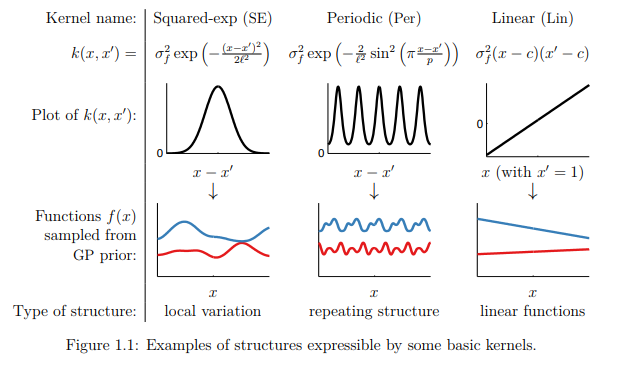
\includegraphics[width=0.7\textwidth]{img/kernels}

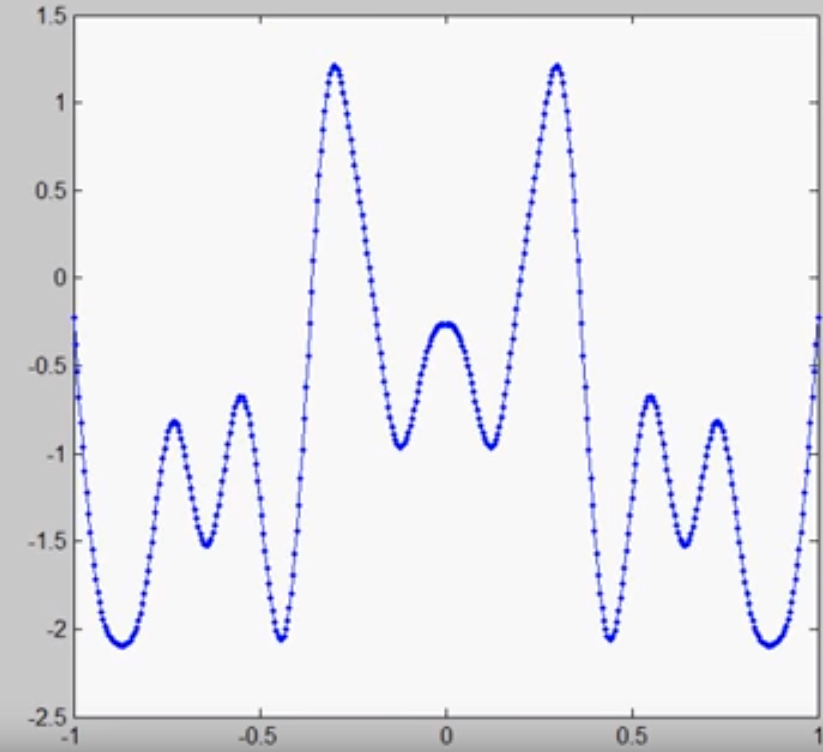
\includegraphics[width=0.7\textwidth]{img/symmetric-kernel}

Image stolen from https://www.cs.toronto.edu/~duvenaud/cookbook/


\begin{tcolorbox}
    \newterm{Gaussian Process} is a \newterm{stochastic process} (a collection of random variables), such that every subset of those random variables has a multivariate Gaussian distribution. It is defined by a mean function $m(x)$ and a covariance funciton $\kappa(x, x')$. Formally, we write \todo{osklive GP}:
    
    \begin{equation}
    f(x) \sim \gN \gG \gP (m(x), \kappa(x, x'))
    \end{equation} \todo{finish}
    
    Bayesian inference ...
    
    \begin{equation}
        \text{posterior} = \frac{\text{likelihood} \times \text{prior}}{\text{evidence}}
    \end{equation},
    
    where evidence is also called \newterm{marginal likelihood}. More concretely, we usually want to compute the posterior distribution over the parameters $\vw$ given the inputs $\mX$ and outputs $\vy$
    
    \begin{equation}
        p(\vw | \vy, \mX) = \frac{p(\vy | \vw, \mX) p(\vw)}{p(\vy | \mX)}
    \end{equation}.
    
    The marginal likelihood is independent of the weights and acts as a normalizing constant. We compute it using marginalization
    
    \begin{equation}
        p(\vy | \mX) = \int p(\vy | \vw, \mX) p(\vw) d \vw.
    \end{equation}
    
    \todo{describe prior over functions}
\end{tcolorbox}


\section{GP from scratch again}



\section{Noise-less Gaussian Process Regression}

\section{Noisy Gaussian Process Regression}


\chapter{TODO Bucket}


\begin{thm}[\citep{murphy2012machine}] (Inverse of a partitioned matrix). Consider a partitioned matrix

\begin{equation}
\mM = \begin{bmatrix} \mA & \mB \\ \mC & \mD \end{bmatrix}
\end{equation}

where we assume $\mA$ and $\mD$ are invertible \todo{staci to? nemusi byt i ty ostatni?}. We have

\begin{equation}
\mM^{-1} = \begin{bmatrix} \mI & \mZero \\ \mI & \mI \end{bmatrix}
\end{equation}
\end{thm}

\begin{proof}
All we need to do is perform a block \newterm{LDU decomposition} and we directly arrive at our solution. We begin by zeroing out $\mB$.

\begin{equation} \label{eq:block-ld-part}
\begin{bmatrix} \mI & -\mB \mD^{-1} & \\ \mZero & \mI \end{bmatrix}
\begin{bmatrix}\mA & \mB \\ \mC & \mD \end{bmatrix} =
\begin{bmatrix} \mA - \mB \mD^{-1} \mC & \mZero \\ \mC & \mD \end{bmatrix}
\end{equation}

The quantity in the top left block is called a \newterm{Schur complement} of $\mM$ wrt $\mD$. We denote it as follows, and also define a variant for the bottom right block

\begin{align}
\mM/\mD &= \mA - \mB \mD^{-1} \mC \\
\mM/\mA &= \mD - \mC \mA^{-1} \mB
\end{align}

Substituting back into \eqref{eq:block-ld-part} we get the following

\begin{equation}
\begin{bmatrix} \mM/\mD & \mZero \\ \mC & \mD \end{bmatrix}
\end{equation}

We follow by eliminating the bottom left block in \eqref{eq:block-ld-part}

\begin{equation} \label{eq:block-du-part}
\begin{bmatrix} \mM/\mD & \mZero \\ \mC & \mD \end{bmatrix}
\begin{bmatrix} \mI & \mZero \\ -\mD^{-1} \mC & \mI \end{bmatrix} =
\begin{bmatrix} \mM/\mD & \mZero \\ \mZero & \mD \end{bmatrix}
\end{equation}

Putting together \eqref{eq:block-ld-part} and \eqref{eq:block-du-part} we get

\begin{equation}
\underbrace{\begin{bmatrix} \mI & -\mB \mD^{-1} & \\ \mZero & \mI \end{bmatrix}}_{\mX}
\underbrace{\begin{bmatrix}\mA & \mB \\ \mC & \mD \end{bmatrix}}_{\mM}
\underbrace{\begin{bmatrix} \mI & \mZero \\ -\mD^{-1} \mC & \mI \end{bmatrix}}_{\mZ} = 
\underbrace{\begin{bmatrix} \mM/\mD & \mZero \\ \mZero & \mD \end{bmatrix}}_{\mW}
\end{equation}

Basic matrix algebra allows us to re-arrange the terms \todo{cite stolen from murphy?}, taking the inverse of both sides

\begin{align}
(\mX \mM \mZ)^{-1} &= \mW^{-1} \\
\mZ^{-1} \mM^{-1} \mX^{-1} &= \mW^{-1} \\
\mM^{-1} &= \mZ \mW^{-1} \mX
\end{align}

Which gives us the final form, making use of the fact that to invert a diagonal matrix we just need to invert its diagonal

\begin{equation} \label{eq:block-inverse}
\mM^{-1} = \begin{bmatrix} \mA & \mB \\ \mC & \mD \end{bmatrix}^{-1} =
\begin{bmatrix} \mI & \mZero \\ -\mD^{-1} \mC & \mI \end{bmatrix}
\begin{bmatrix} (\mM/\mD)^{-1} & \mZero \\ \mZero & \mD^{-1} \end{bmatrix}
\begin{bmatrix} \mI & -\mB \mD^{-1} & \\ \mZero & \mI \end{bmatrix}
\end{equation}

\end{proof}



\section{TODO Linear Gaussian transform - change of variables}

\begin{align}
P(\vx \in \mM) = \int_\mM \frac{1}{(2 \pi)^{D/2} |\mSigma|^{1/2}|} exp \left(-\frac{1}{2} (\vx - \vmu)^T \mSigma^{-1} (\vx - \vmu) \right) d \vx \\
P(\vx \in \mA^{-1} \mM) = \int_{\mA^{-1} \mM} \frac{1}{(2 \pi)^{D/2} |\mSigma|^{1/2}} \exp \left(-\frac{1}{2} (\vu - \vmu)^T \mSigma^{-1} (\vu - \vmu) \right) d \vu \\
\vu = \mA \vx
\end{align}

